\documentclass[tikz,border=10pt]{standalone}
\usepackage{amsmath}
\begin{document}
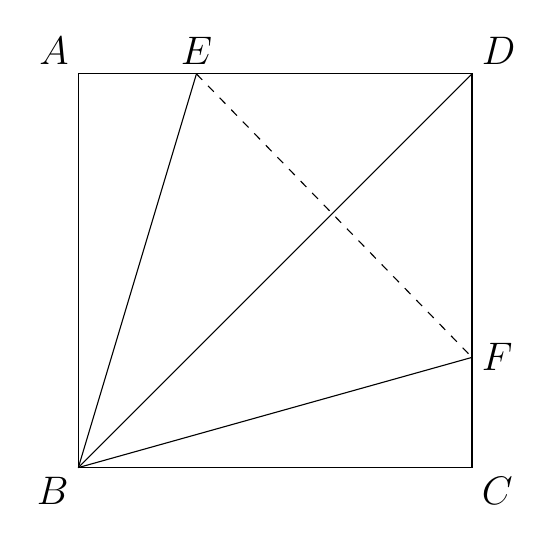
\begin{tikzpicture}[scale=1, font=\Large]
  % Square vertices
  \coordinate (A) at (0,5);
  \coordinate (D) at (5,5);
  \coordinate (C) at (5,0);
  \coordinate (B) at (0,0);

  % Points on the sides
  \coordinate (E) at (1.5,5);
  \coordinate (F) at (5,1.4);

  % Square outline
  \draw (A) -- (D) -- (C) -- (B) -- cycle;

  % Solid edges
  \draw (B) -- (E);
  \draw (B) -- (D);
  \draw (B) -- (F);

  % Dashed edge
  \draw[dashed] (E) -- (F);

  % Labels
  \node[above left] at (A) {$A$};
  \node[above right] at (D) {$D$};
  \node[below right] at (C) {$C$};
  \node[below left] at (B) {$B$};
  \node[above] at (E) {$E$};
  \node[right] at (F) {$F$};
\end{tikzpicture}
\end{document}
